\subsection{Neurons}
The term \textbf{neural network} (NN) is a reference to the workings of nervous systems of humans \cite{NeuralNetworkLiteratureReview}. These systems consist of a net of neurons, biological cells that are intricately connected to other neurons through structures called synapses \cite{PrinciplesOfBrainFunctioningHaken}. These connections carry electric pulses between neurons that can excite them when those pulses exceed certain thresholds. Those thresholds vary from neuron to neuron and change over time. Upon excitation, new pulses in turn propagate from the excited neuron outwards to possibly excite other neurons. This interplay between excitation and transmission through the network of neurons may create what we perceive as thinking.\\
In attempts to eventually understand and replicate this thinking process, mathematical analyses of such systems  have been done as early as the 1940's \cite{A_logical_calculus_of_the_ideas_immanent_in_nervous_activity}. The artificial neural networks used in machine learning today are mathematical concepts that replicate the transmission of excitation between neurons. To examine how this is achieved using mathematical functions and values instead of biological cells and electric pulses, let's look at how the artificial neural networks are built.\\
The \textbf{neurons}, which function as building blocks of artificial neural networks, are mathematical entities that take a fixed number of scalar values as inputs and convert them into a single output value. For a more visual explanation let's take a look at \cref{fig:Neuron_explanation}, which illustrates the example of a neuron with 2 inputs.
\begin{figure}
	\centering
	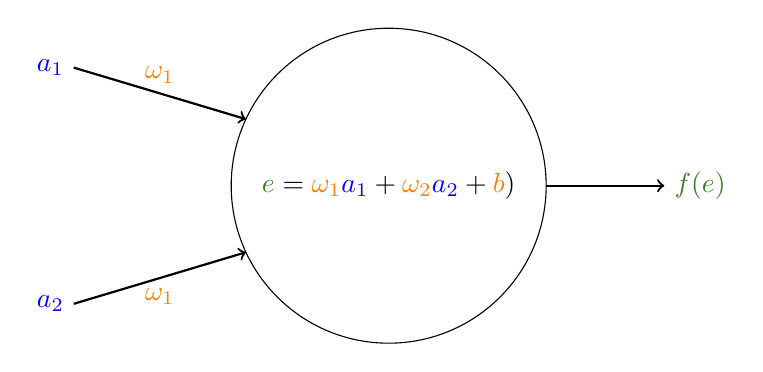
\begin{tikzpicture}[shift={(0,0)}]
	\draw (5,5) circle[radius=2];
	
	% Calculate the coordinates on the circle's circumference
	\pgfmathsetmacro\arrowOneX{5 + cos(155) * 2} % 45 degrees angle
	\pgfmathsetmacro\arrowOneY{5 + sin(155) * 2}
	
	\pgfmathsetmacro\arrowTwoX{5 + cos(-155) * 2} % 135 degrees angle
	\pgfmathsetmacro\arrowTwoY{5 + sin(-155) * 2}
		
	\draw[->, thick] (1,6.5) -- (\arrowOneX, \arrowOneY) node[pos=0.5,above] {$\textcolor{orange}{\omega_1}$};
	\draw (1,6.5) node[left] {$\textcolor{blue}{a_1}$};
	\draw[->, thick] (1,3.5) -- (\arrowTwoX, \arrowTwoY) node[pos=0.5,below] {$\textcolor{orange}{\omega_1}$};
	\draw (1,3.5) node[left] {$\textcolor{blue}{a_2}$};
	\node at (5,5) {$\textcolor{OliveGreen}{e} = \textcolor{orange}{\omega_1}\textcolor{blue}{a_1} + \textcolor{orange}{\omega_2}\textcolor{blue}{a_2} + \textcolor{orange}{b})$};	
	\draw[->, thick] (7,5) -- (8.5,5) node[right] {$\textcolor{OliveGreen}{f(e)}$};
	
	
\end{tikzpicture}
	\caption{This figure aids the explanation of the operating principle of neurons in neural networks. The weights $\omega_i$ and the bias $b$ are denoted in orange, the input activations $a_i$ in blue and the activation $e$ with its corresponding activation function $f$ in magenta.}
	\label{fig:Neuron_explanation}
\end{figure}
The big circle in the middle represents the neuron itself. It takes the activation values $a_i$ as input, multiplies them with their corresponding weights $\omega_i$, sums them up, and adds a bias value $b$ to obtain the excitation $e$. It then applies the activation function onto $e$ to obtain the resulting output value. The input activations $a_i$ correspond to the strength of electronic pulses in the nervous system. The absence of a pulse in the biological system would be represented by an activation of zero in the mathematical model. The weights $\omega_i$ are a representation of how important single input values are for the activation of the neuron. In the biological counterpart this might correspond to how thick or conductive the connections between the nerve cells are. Finally, the combination of bias $b$ and activation function determines how large the sum of the input-weight-pairs has to be to activate the neuron and how the resulting value for the activation of the neuron changes for higher input activations. For example, a simple output activation function would be the ReLU function (Rectified Linear Unit).
This function is defined as \cite{ActivationFunctionOverview}
\begin{equation}
	f(x) = 
	\begin{cases}
		x, &\text{if } x\geq0 \\
		0, &\text{otherwise}
	\end{cases}.
\end{equation} 
When applying a ReLU activation function, the neuron is activated as soon as the sum of the input-weight-pairs is larger than $-b$. Its value increases linearly with $e$.
\subsection{Neural networks}\label{sec:NeuralNetworks}
A neural network can be built from these neurons by connecting the outputs of neurons to the inputs of others. An example of such a network is illustrated in \cref{fig:Neural_network_example}. This neural network consists of three layers of four neurons each, takes two values as input and outputs one value. For example, it could be used as an approximator of whether a point on a 2D-grid is inside or outside of a given region. The input values would be the $x$ and $y$ coordinates of the point and the output value could represent the predicted probability that the point is inside this region. How to find parameters that make the network correctly classify a desired region will be explained in \cref{sec:NeuralNetworkTraining}.\\
\begin{figure}
	\centering
	\begin{tikzpicture}
	\Vertex[x=0,y=0]{A}
	\Vertex[x=0,y=1]{B}
	\Vertex[x=0,y=2]{C}
	\Vertex[x=0,y=3]{D}
	
	\Vertex[x=2,y=0]{E}
	\Vertex[x=2,y=1]{F}
	\Vertex[x=2,y=2]{G}
	\Vertex[x=2,y=3]{H}
	
	\Vertex[x=4,y=0]{I}
	\Vertex[x=4,y=1]{J}
	\Vertex[x=4,y=2]{K}
	\Vertex[x=4,y=3]{L}
	
	\Edge[lw=1pt](A)(E)
	\Edge[lw=1pt](A)(F)
	\Edge[lw=1pt](A)(G)
	\Edge[lw=1pt](A)(H)
	
	\Edge[lw=1pt](B)(E)
	\Edge[lw=1pt](B)(F)
	\Edge[lw=1pt](B)(G)
	\Edge[lw=1pt](B)(H)
	
	\Edge[lw=1pt](C)(E)
	\Edge[lw=1pt](C)(F)
	\Edge[lw=1pt](C)(G)
	\Edge[lw=1pt](C)(H)
	
	\Edge[lw=1pt](D)(E)
	\Edge[lw=1pt](D)(F)
	\Edge[lw=1pt](D)(G)
	\Edge[lw=1pt](D)(H)
	
	\Edge[lw=1pt](E)(I)
	\Edge[lw=1pt](E)(J)
	\Edge[lw=1pt](E)(K)
	\Edge[lw=1pt](E)(L)
	
	\Edge[lw=1pt](F)(I)
	\Edge[lw=1pt](F)(J)
	\Edge[lw=1pt](F)(K)
	\Edge[lw=1pt](F)(L)
	
	\Edge[lw=1pt](G)(I)
	\Edge[lw=1pt](G)(J)
	\Edge[lw=1pt](G)(K)
	\Edge[lw=1pt](G)(L)
	
	\Edge[lw=1pt](H)(I)
	\Edge[lw=1pt](H)(J)
	\Edge[lw=1pt](H)(K)
	\Edge[lw=1pt](H)(L)
	
	\Vertex[x=-2,y=1, label=$x$, opacity = 0]{X}
	\Vertex[x=-2,y=2, label=$y$, opacity = 0]{Y}
	\Edge[lw=1pt](X)(A)
	\Edge[lw=1pt](X)(B)
	\Edge[lw=1pt](X)(C)
	\Edge[lw=1pt](X)(D)
	\Edge[lw=1pt](Y)(A)
	\Edge[lw=1pt](Y)(B)
	\Edge[lw=1pt](Y)(C)
	\Edge[lw=1pt](Y)(D)
	
	\Vertex[x=6,y=1.5, label=$p$, opacity = 1]{P}
	\Edge[lw=1pt](I)(P)
	\Edge[lw=1pt](J)(P)
	\Edge[lw=1pt](K)(P)
	\Edge[lw=1pt](L)(P)
	
	\draw [decorate,
	decoration = {brace, mirror, amplitude=10pt}] (-0.2,-0.5) --  (4.2,-0.5);
	\node at (2,-1.2) {3 (hidden) layers};
	\draw [decorate,
	decoration = {brace, mirror, amplitude=10pt}] (6.5,-0.3) --  (6.5,3.3);
	\node at (7.2,1.5) [rotate=-90] {width of 4 neurons};
	
\end{tikzpicture}
	\caption{This figure shows an example of a neural network. It consists of multiple neurons connected to each other. This network takes in 2 input values and returns one output value. It consists of 3 hidden layers, each having a width of 4 neurons.}
	\label{fig:Neural_network_example}
\end{figure}
This network serves as an illustrative example, showing what a neural network can look like. For real-world applications, there are various kinds of networks used to learn different tasks \cite{DeepLearningTaxonomy}. For this thesis we will only talk about "fully connected" or "dense" neural networks. This means that every neuron in the first layer will receive every possible network input value, and every neuron in later layers will receive the output of every neuron in the previous layer as input. All neurons are equipped with the same activation function. The weights and biases vary throughout. How the output of the network gets handled may still differ through different use cases. \\
When working on classification tasks, it can be beneficial to feed the output of the neural network into a so-called softmax function before analyzing it. This function converts the scalar outputs of the network, which can be any number from $\mathbb{R}$, into probabilities of the inputs belonging to specific classes. These aren't real probabilities, since every input\footnote{The term input can refer to single scalar values given to neurons, as well as to whole sets of scalar values given to the network.} belongs to a predefined class, but rather represent the network's confidence in the predicted classifications. For a set of outputs $z_i$, the standard softmax function is defined as 
\begin{equation}\label{eq:softmax}
	\sigma_i(z) = \frac{\mathrm{exp}(z_i)}{\sum_j \mathrm{exp}(z_j)}.
\end{equation}
The resulting values lie between $0$ and $1$ and add up to a total of $1$. A larger value of an output node results in a higher corresponding probability. For further details on the softmax function, see \cite{gao2018properties}.\\
The structure of a neural network is generally referred to as the \textbf{architecture} of the network, with the hidden layers\footnote{We also sometimes simply refer to hidden layers as layers.} referring to the columns of neurons in between the input values and output neurons and the amount of neurons per layer referred to as the "width" of the network. This is also denoted in \cref{fig:Neural_network_example}. 
\subsection{Mathematical view}
The previous explanations have been very visual and step by step to make the topic more accessible. However, these concepts can be broken down to rather short mathematical expressions.\\
To start off, we can define the inputs as $a_i^{(0)}$ , $i =  1, \ldots, n$. The weights of the first hidden layer can be denoted by $\omega_{i}^{(1)}$, $i =  1, \ldots, n$. Furthermore, we define $\omega_{i,j}^{(k)}$ as the weight that connects the $i$-th neuron in the $k$-th layer to the $j$-th neuron in the $(k-1)$-th layer. The maximum values of $i$ and $j$ depend on the widths of the respective layers, $k$ can reach values between $1$ and the amount of hidden layers plus 1. The bias of the $i$-th neuron in the $k$-th layer is denoted as $b_i^{(k)}$. Using this notation we can write out the output of the $i$-th neuron in the $(k+1)$-th layer as \cite{NeuralNetworksBook}
\begin{equation}
	a_i^{(k+1)} = f\left(\sum_j \left(\omega_{i,j}^{(k+1)}a_j^{(k)}\right) + b_i^{(k+1)}\right).
\end{equation}
To actually calculate this value, the activations $a_j^{(k)}$ have to be recursively replaced with their full calculation until one arrives at the input values of the network.\\
For simplicity reasons, we will refer to the weights $\omega_{i,j}^{(k)}$ and biases $b_i^{(k)}$ together as \textbf{parameters} of the neural network. We will denote these collected in one ordered set as $\theta = \{\theta_i\}_{i=1}^{N}$, where $N$ is the total number of weights and biases added together. The mapping of the parameters onto $\theta$ can be arbitrarily chosen. When talking about all parameters as a single set, the corresponding mapping has to be known, so that it's possible to calculate the output of the network when given the parameters in the same way as when given the actual weights and biases. Another possible representation that we will use often is to write this set as a vector $\theta \in \mathbb{R}^N$. A short notation for the output of the neural network will be explained in the next section.
